\section{Case Study}
\label{sec:casestudy}
This section describes the scenarios that demonstrate the use of the testbed proposed in this paper. In particular, we consider two scenarios separately to demonstrate the effect of network attacks. The adversarial attacks we demonstrate include Data Integrity Attacks (DIA) and Denial of Service Attacks (DoS). Table \ref{tab:attacks_comparison} highlights the key differences between the two attack types.
% \begin{itemize}
%     \item \textbf{Data Integrity Attacks (DIA) }are cyberattacks where an unauthorized party illicitly modifies the data stored, processed, or in transit within a system, thus compromising its accuracy and reliability. 
%     \item \textbf{Data Denial of Service Attacks (DoS)} target the availability of a service, intending to overwhelm the resources of a system, such as servers or networks, making it inaccessible to legitimate users
% \end{itemize}
% Table \ref{tab:attacks_comparison} summarizes the unique characteristics of the two attack types.
\begin{table}[!ht]
% \vspace{-0.3cm}
\centering
\caption{Attack comparison}
% \vspace{-0.3cm}
\label{tab:attacks_comparison}
\begin{tabular}{@{}>{\raggedright}p{0.2\linewidth}>{\raggedright\arraybackslash}p{0.35\linewidth}>{\raggedright\arraybackslash}p{0.35\linewidth}@{}}
\toprule
\textbf{Aspect} & \textbf{Data Integrity Attacks (DIA)} & \textbf{Denial of Service (DoS) Attacks} \\
\midrule
Primary Objective & Alter or corrupt data to undermine its accuracy and reliability. &  Make a network or service unavailable to its intended users. \\
% \addlinespace
% Impact on Services & Damages the correctness of information, leading to potential misuse. & Disrupts service availability, causing downtime and inaccessibility. \\
% \addlinespace
% Typical Methods & Malware, SQL injection, phishing, exploiting software vulnerabilities. & DoS attacks (distributed denial of service), SYN floods, ping of death, etc. \\
\addlinespace
Target & Data stored, in transit, or being processed. & Network infrastructure and servers. \\
\addlinespace
Detection & Requires monitoring for unauthorized data changes or anomalies. & Can often be detected by monitoring for sudden spikes in traffic. \\
% \addlinespace
% Goal of Attacker & To mislead, cause harm, or perpetrate fraud. & To disrupt operations, often for protest or to demand ransom. \\
\bottomrule
\end{tabular}
% \vspace{-0.6cm}
\end{table}

% We demonstrate the effect of these attacks on both the Power grid and Chemical Plant.

\subsection{Attacks on Power grid.}
The attacks on the Power Grid  include DoS and False Data Injection (FDI), which can be instigated at the communication path between any of the \textit{LC}s and the \textit{SC}. An adversary that succeeds in gaining control of the host machine becomes capable of manipulating the information transferred between the controllers or jamming the bandwidth to deny the information exchange between the controllers over the Mininet topology.  For demonstration purposes, we mimic the attacker behavior using a python script that will interfere with the functioning of each of these controllers. For DIA using FDI attack, we target the information being sent from the controllers (\textit{SC} or \textit{LC}) and manipulate it by running a script in parallel that will replace this data while ensuring higher priority/rank for the substation.
\begin{figure}[!ht]
% \vspace{-0.2cm}
    \centering
    
\includegraphics[width=\linewidth]{Figures/legend_only.pdf} \\
%     \vspace{-0.1cm}
    \definecolor{dark_contrast}{HTML}{006400}
    \def\linenda{0.987}
    \def\linendb{0.987}
    \begin{tikzpicture}
        \node[anchor=south west,inner sep=0] (image) at (0,0) {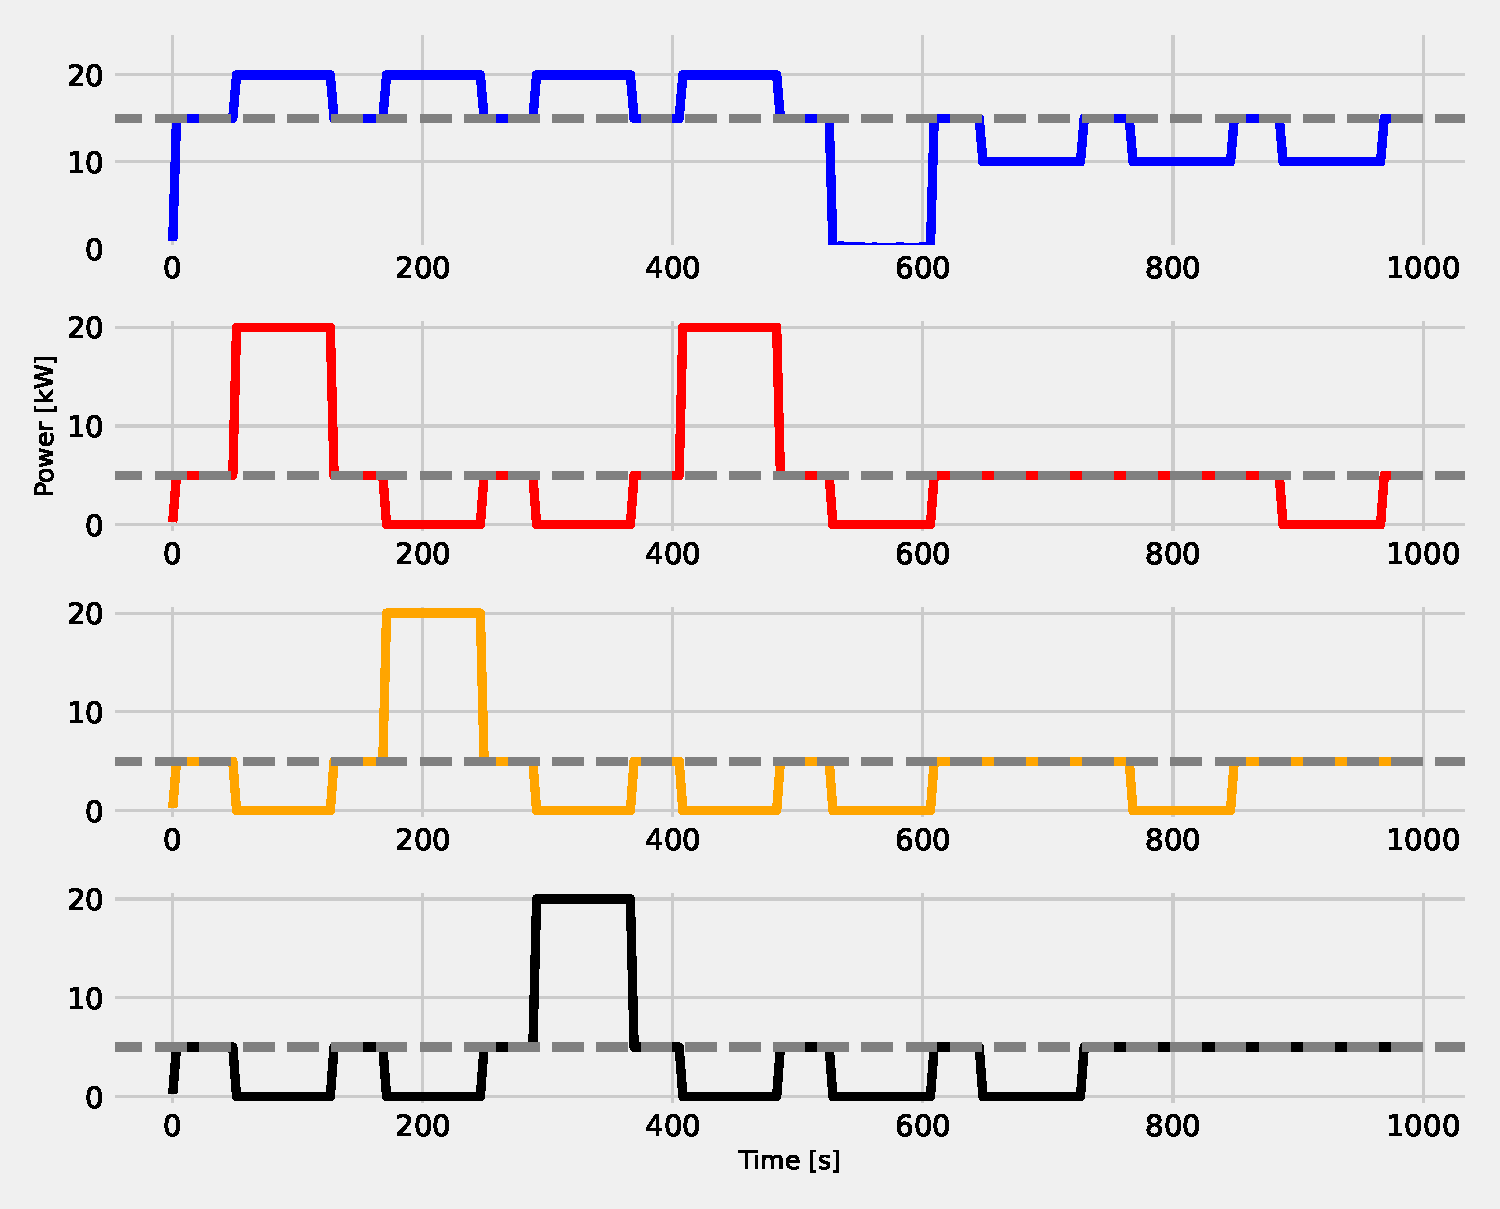
\includegraphics[width=\linewidth]{Figures/demand_and_supply.pdf}};
        \begin{scope}[x={(image.south east)},y={(image.north west)}]
            \draw [dark_contrast, thick, dashed, line width=0.75pt] (0.156,0) -- (0.156,\linenda) node [above, black] {};
            \draw [dark_contrast, thick, dashed, line width=0.75pt] (0.222,0) -- (0.222,\linenda);
            \node[red, text width=3cm, align=center] at (0.19,1) {\tiny{FDI-$lc_1$}};
            
            \draw [dark_contrast, thick, dashed, line width=0.75pt] (0.256,0) -- (0.256,\linendb) node [above, black] {};
            \draw [dark_contrast, thick, dashed, line width=0.75pt] (0.322,0) -- (0.322,\linendb);
            \node[red, text width=3cm, align=center] at (0.29,1) {\tiny{FDI-$lc_2$}};

            \draw [dark_contrast, thick, dashed, line width=0.75pt] (0.356,0) -- (0.356,\linenda) node [above, black] {};
            \draw [dark_contrast, thick, dashed, line width=0.75pt] (0.422,0) -- (0.422,\linenda);
            \node[red, text width=3cm, align=center] at (0.39,1) {\tiny{FDI-$lc_3$}};

            \draw [dark_contrast, thick, dashed, line width=0.75pt] (0.456,0) -- (0.456,\linendb) node [above, black] {};
            \draw [dark_contrast, thick, dashed, line width=0.75pt] (0.522,0) -- (0.522,\linendb);
            \node[red, text width=3cm, align=center] at (0.49,1) {\tiny{FDI-$sc$}};

            \draw [dark_contrast, thick, dashed, line width=0.75pt] (0.556,0) -- (0.556,\linenda) node [above, black] {};
            \draw [dark_contrast, thick, dashed, line width=0.75pt] (0.622,0) -- (0.622,\linenda);
            \node[red, text width=3cm, align=center] at (0.59,1) {\tiny{DoS-$sc$}};

            \draw [dark_contrast, thick, dashed, line width=0.75pt] (0.656,0) -- (0.656,\linendb) node [above, black] {};
            \draw [dark_contrast, thick, dashed, line width=0.75pt] (0.722,0) -- (0.722,\linendb);
            \node[red, text width=3cm, align=center] at (0.69,1) {\tiny{DoS-$lc_3$}};

            \draw [dark_contrast, thick, dashed, line width=0.75pt] (0.756,0) -- (0.756,\linenda) node [above, black] {};
            \draw [dark_contrast, thick, dashed, line width=0.75pt] (0.822,0) -- (0.822,\linenda);
            \node[red, text width=3cm, align=center] at (0.79,1) {\tiny{DoS-$lc_2$}};        

            \draw [dark_contrast, thick, dashed, line width=0.75pt] (0.856,0) -- (0.856,\linendb) node [above, black] {};
            \draw [dark_contrast, thick, dashed, line width=0.75pt] (0.922,0) -- (0.922,\linendb);
            \node[red, text width=3cm, align=center] at (0.89,1) {\tiny{DoS-$lc_1$}};
        % \draw [rounded corners, thick] (0.05,-0.03) rectangle (0.95,0.01);
        %     \node at (0.5,-0.015) {\tiny{FDI: False Data Injection, DoS: Denial of Service, $lc_{i}$: local controller $i$, sc: supervisory controller}};    
        \end{scope}
    \end{tikzpicture}
%     \vspace{-0.5cm}
    \caption{Visualization of demand and supply values under attacks. FDI and DoS correspond to the False Data Injection and Denial of Service respectively, while $lc_i$ and $sc$ depicts  the attacked local and supervisory controllers respectively. }
    \label{fig:grid_attack}
%     \vspace{-0.1cm}
\end{figure}
  For instance, if the local controller associated with substation 1, \textit{LC}1, demands a higher power beyond the power grid capacity (20kW) at the highest priority, then \textit{LC}2 and \textit{LC}3 (requesting a steady 5kW for the next sampling interval) are forced to send their respective substations to island mode. Figure \ref{fig:grid_attack} shows the demand and supply of the \textit{SC} and \textit{LC}s under the FDI attacks on each of the controllers. 
  The first four annotations in the Figure correspond to FDI attacks on \textit{LC}1, \textit{LC}2, \textit{LC}3, and the \textit{SC} respectively. 

To replicate a DoS attack, a Python script running in parallel threads disrupts communication between Local Controllers and the Supervisory Controller. This interruption prevents information from reaching its intended destination, effectively blocking updates. As a result, in the absence of communication, the system interprets the missing data as 0 kW demand (from an \textit{LC}) or 0 kW supply (from the \textit{SC}), causing the affected substation to enter islanding mode. The impact of this attack is visualized through plots in Figure \ref{fig:grid_attack} where
the last four annotations illustrate DoS attacks targeting the \textit{SC}, \textit{LC}3, \textit{LC}2, and \textit{LC}1, respectively. 

Each attack type exhibits a distinct supply-demand pattern, which can be compared against the actual demand and supply values recorded at the GridLAB-D logs. This comparison is the key observation for attack detection and type.The current stage of this test bed features only one actuator (a load switch for islanding) for power regulation. We manually regulate the load module within GridLAB-D to adjust the load value and maintain a constant voltage for the power supplied. In the future, this will be improved by adding more ZIP loads connected to the substation, equipped with custom switches that can modify the overall load. This enhancement will provide more granular observations beyond the discrete levels depicted in Figure \ref{fig:grid_attack}.



% \begin{figure}[H]
%     % First row
%     \begin{subfigure}{0.5\linewidth}
%         \hspace*{-1.5cm} % Adjust the value as needed to shift the image to the left
%         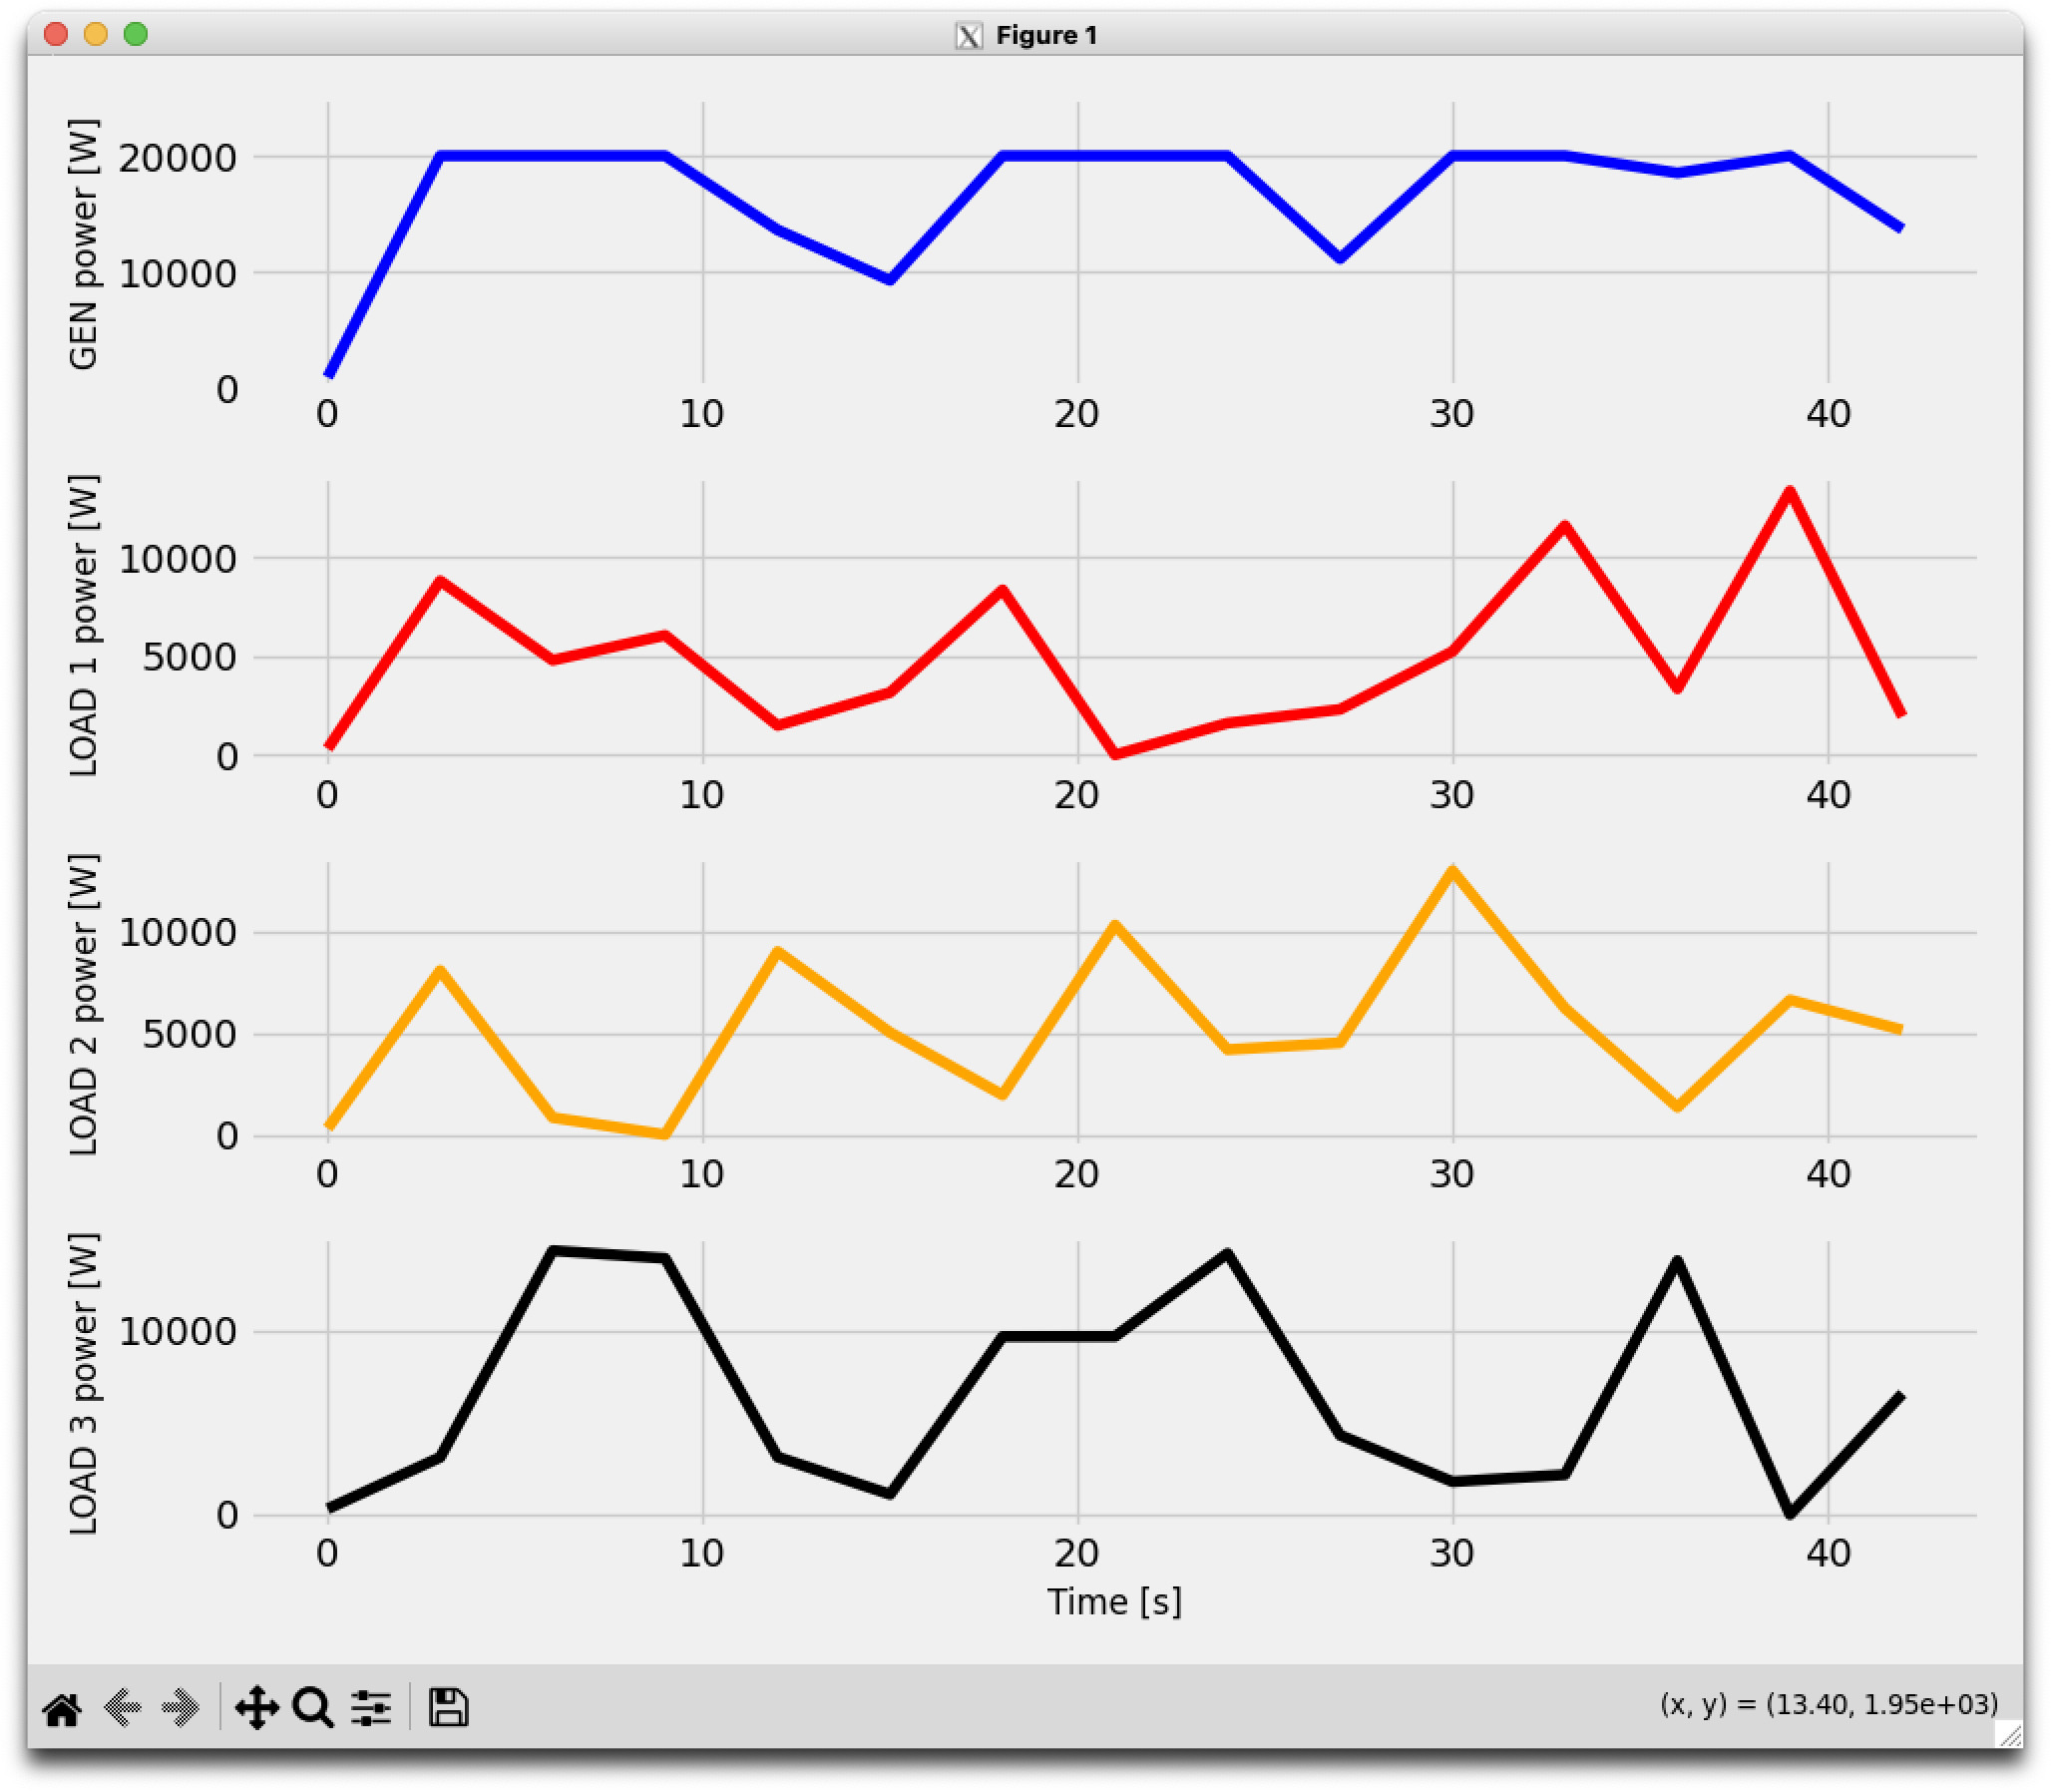
\includegraphics[width=8cm,keepaspectratio]{Figures/normal_mode.png}
%         \caption{}
%         \label{fig:no_attack}
%     \end{subfigure}
%     % You may remove the vspace if you don't need extra vertical space between the subfigures
%     \vspace{1cm} 
%     \begin{subfigure}{0.5\linewidth}
%         \hspace*{-1.5cm} % Adjust the value as needed to shift the image to the left
%         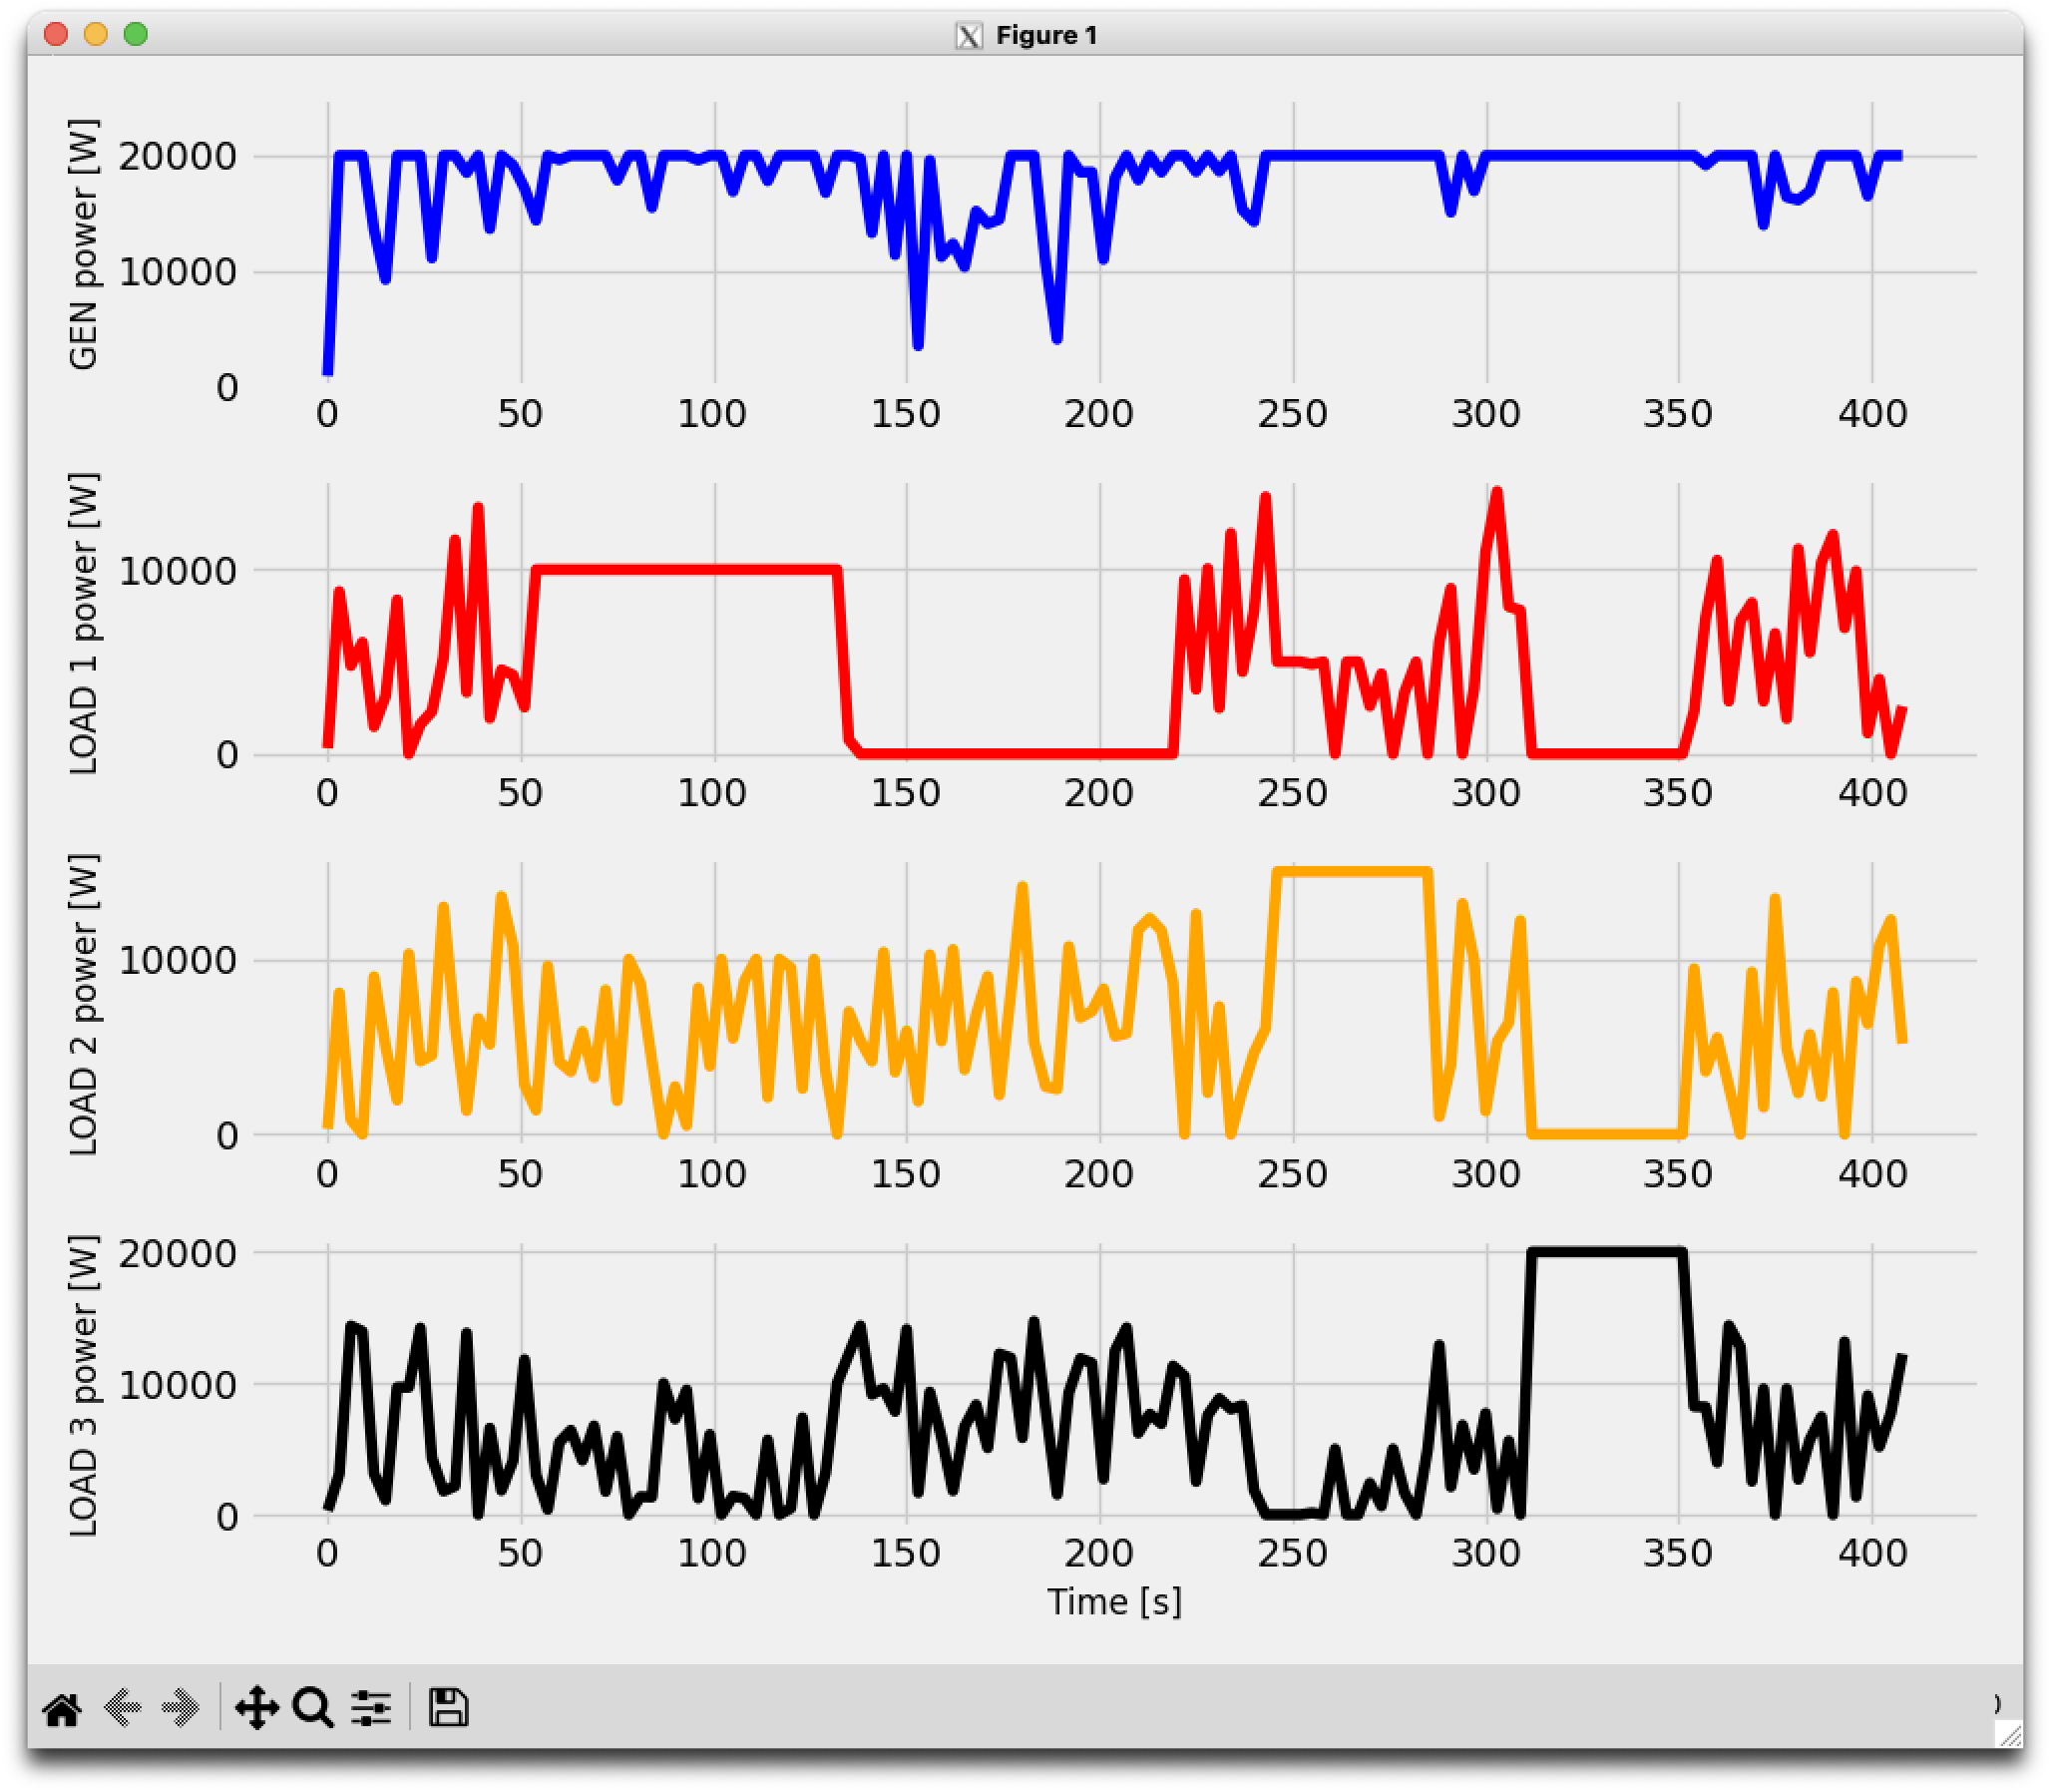
\includegraphics[width=8cm,keepaspectratio]{Figures/different_attacks.png}
%         \caption{}
%         \label{fig:with_attack}
%     \end{subfigure}
%     \caption{Different stages in the power grid attack resulting in islanding.}
%     \label{fig:grid_attack}
% \end{figure}


% \begin{figure}
%         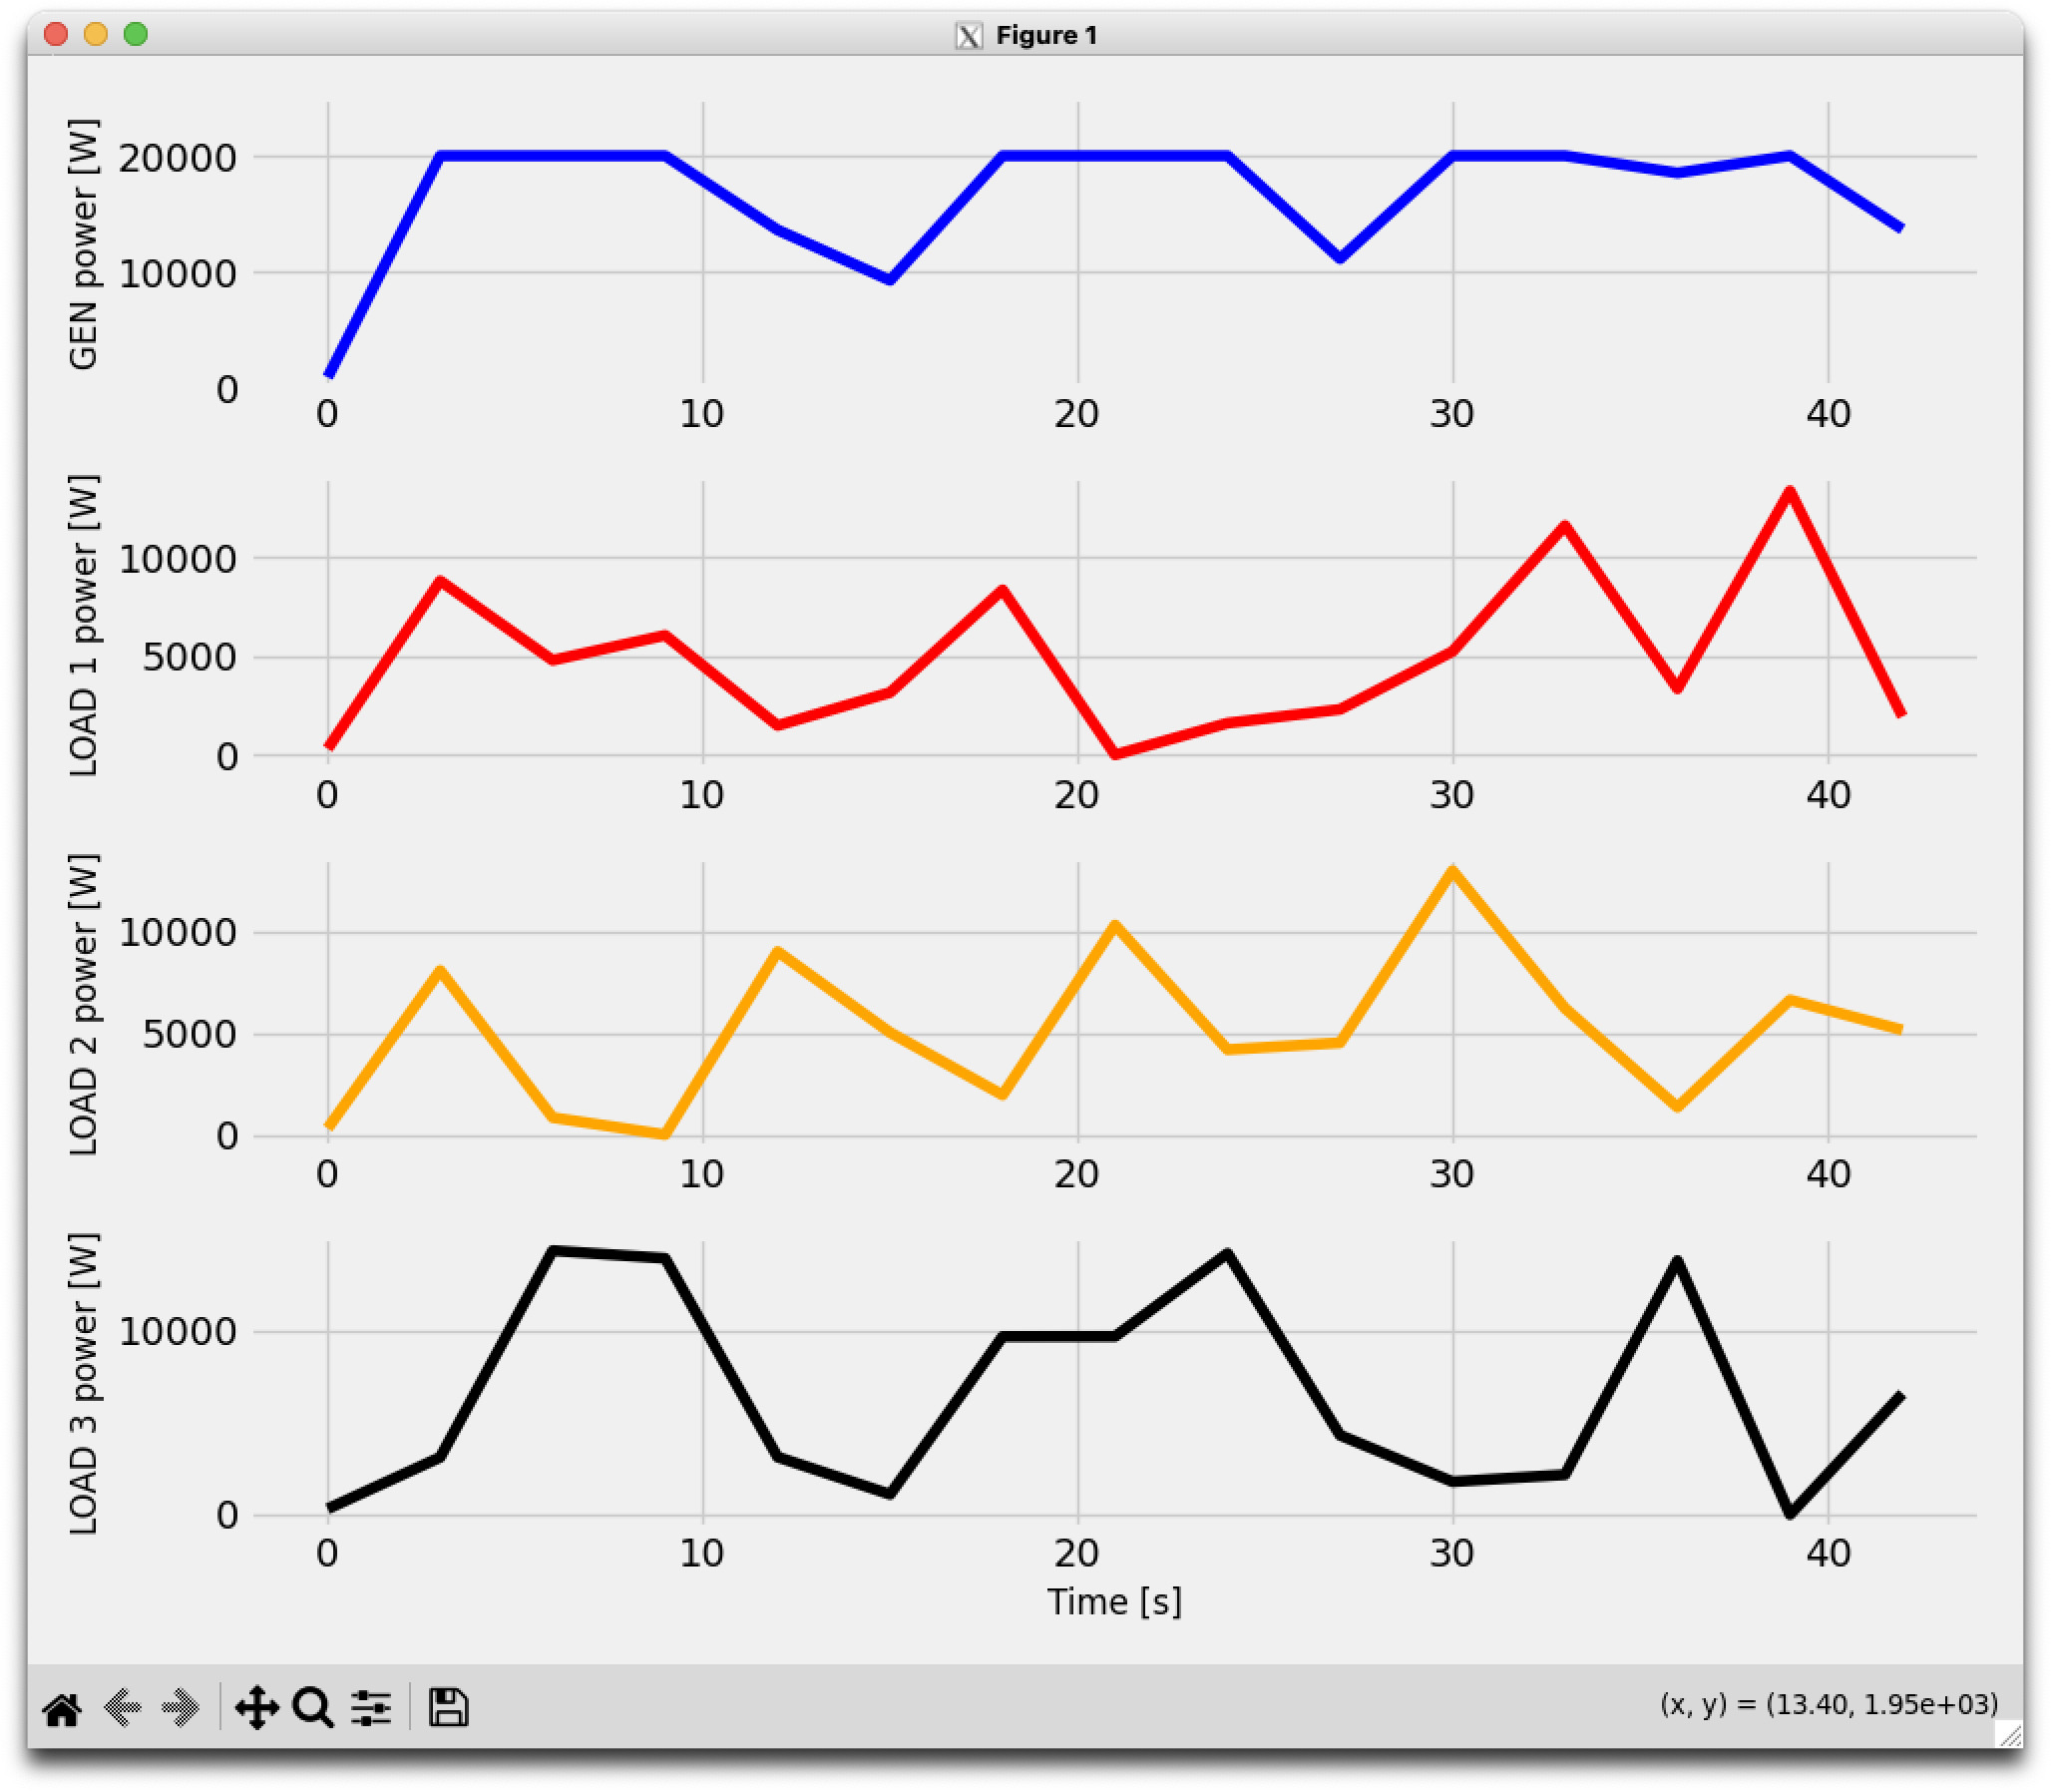
\includegraphics[width=8cm,keepaspectratio]{Figures/normal_mode.png}
%         \caption{}
%         \label{fig:no_attack}
% \end{figure}




\subsection{Attacks on Chemical Plant}
% \begin{figure}[H]
% \begin{tikzpicture}
%     \node[draw, rectangle, rounded corners, minimum width=3.5cm, minimum height=1.5cm, fill=blue!30] (rect1) {};
%     \node[label={[yshift=0.2cm]north:Chemical Plant}] at (rect1.center) {};
    
%     \foreach \x [count=\xi] in {1,...,6} {
%         \coordinate (square-\xi) at ([xshift=-0.2cm + \x*0.5cm, yshift=0.5cm] rect1.south west);
%         \draw (square-\xi) rectangle ++(0.4cm,0.4cm);
%     }
%     \foreach \x in {1,...,6} {
%         \draw[fill=gray] ([xshift=-0.2cm + \x*0.5cm, yshift=0.5cm] rect1.south west) rectangle ++(0.4cm,0.4cm);
%     }
%         \draw[thick, dotted, -Latex] ([xshift=0.25cm, yshift=0.25cm]square-1) to[bend left] ([xshift=-1cm, yshift=1cm]square-1) node[anchor=south west, fill=white] {Sensor};


%     \node[draw, rectangle, rounded corners, minimum width=3.5cm, minimum height=1.5cm, fill=red!30, below=1cm of rect1] (rect2) {Master PLC};
%     \coordinate (top point) at ([xshift=4cm,yshift=0cm] rect1.north);
%     \coordinate (bottom point) at ([xshift=4cm,yshift=0cm] rect2.south);

%     \node[draw, rectangle, minimum width=4cm, minimum height=0.5cm, fill=green!30, rotate=270, right=1cm of rect1.east |-
%     rect2.east] (longrect) at ($(top point)!0!(bottom point)$) {Control Network};



% \foreach \x in {1,...,6} {
%     \ifodd\x\relax
%         \draw[Latex-Latex] (rect2.north) -- ($(square-\x.south)+(0.2,0cm)$);
%     \else
%         \draw[thick, dotted, Latex-Latex] (rect2.north) -- ($(square-\x.south)+(0.2,0cm)$);
%     \fi
% }
%     \draw[thick, {Latex[length=2mm]}-{Latex[length=2mm]}] (rect1.east) -- ($(longrect.south)+(0cm,1.25cm)$);
%     \draw[thick, {Latex[length=2mm]}-{Latex[length=2mm]}] (rect2.east) -- ($(longrect.south)+(0cm,-1.25cm)$);
% \end{tikzpicture}
%     \caption{Schematic depicting the chemical plant under availability attacks. The dotted arrows between the plant and plc are the sensor information blocked as a consequence of the attack.}
%     \label{fig:Chemical_DoS}
%     \Description{DoS chemical plant attack}
% \end{figure}
Figure \ref{fig:Chemical_attacks} shows the schematic of the attack implementations on the Chemical Plant. An attacker gaining access to the hosts can initiate these attacks by intercepting the information sent and received between the PLC and the plant.   
% \begin{figure}
%     \centering
%     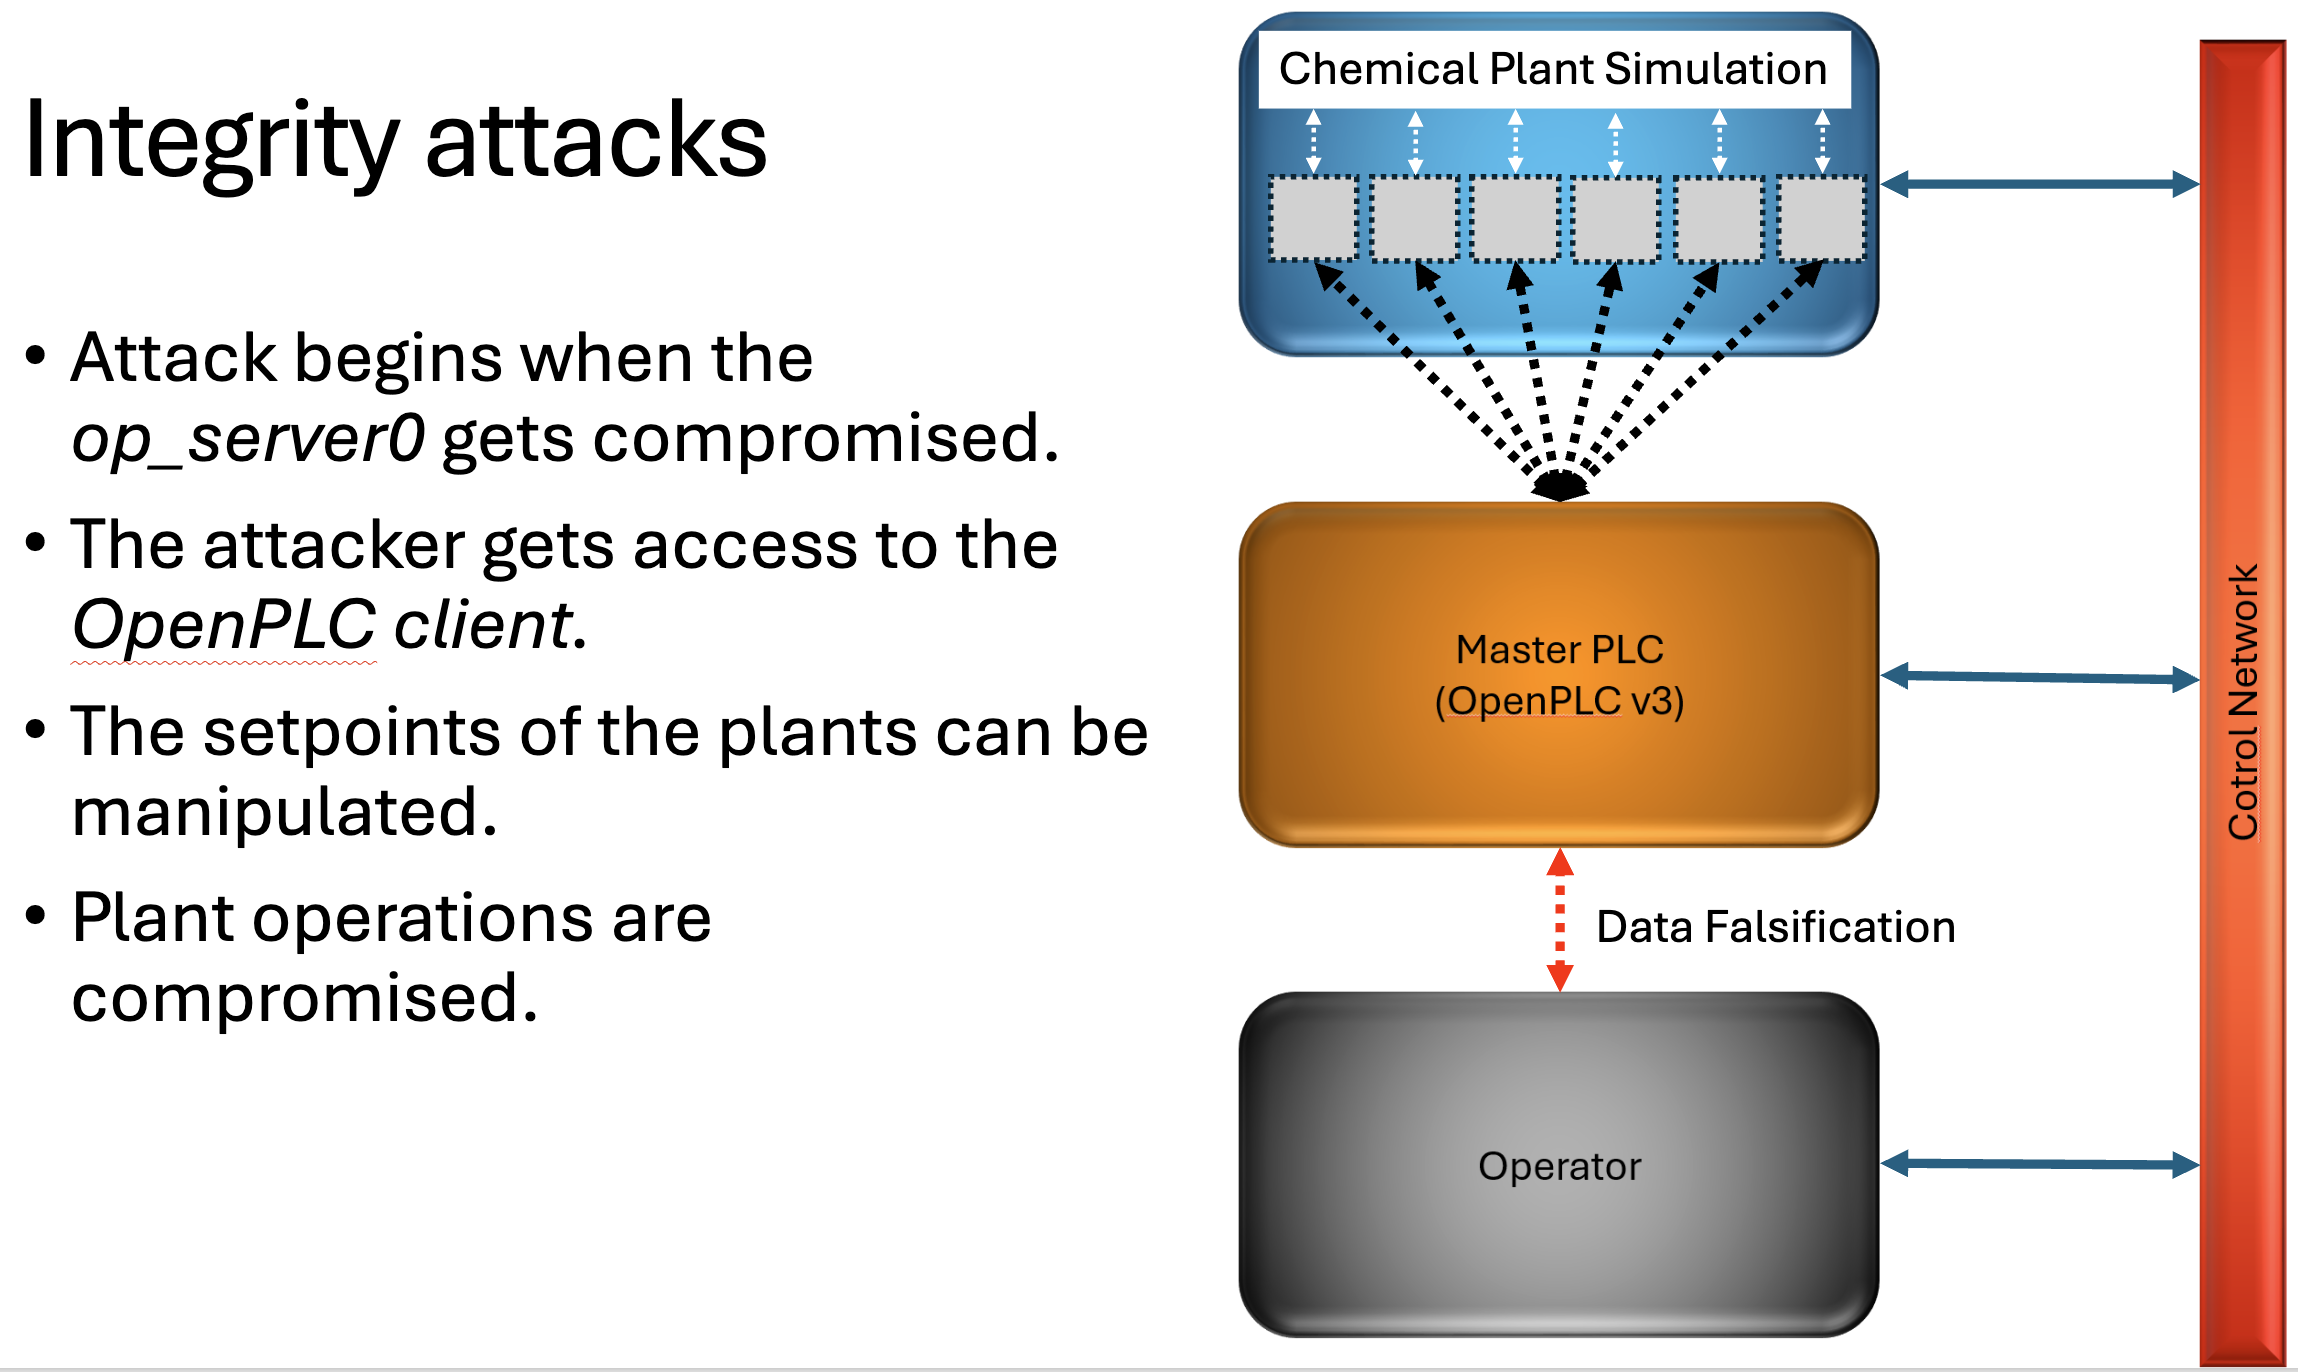
\includegraphics[width=\linewidth]{Figures/ChemicalPlantIntegrity.png}
%     \caption{Schematic showing the chemical plant under integrity attacks.}
%     \label{fig:Chemical_DIA}
% \end{figure}
\begin{figure}[!htbp]
\centering
\begin{tikzpicture}[decoration={brace,amplitude=10pt}]
    % Chemical Plant (left): tall box, "Chemical Plant" horizontal at bottom
    \node[draw, rectangle, rounded corners, minimum width=2.5cm, minimum height=4.0cm, fill=blue!30] (rect1) {};
    \node[font=\small] at ([yshift=0.22cm] rect1.south) {Chemical Plant};

    % PLC slave squares: sq-\y = bottom-left, sqc-\y = centre of each square
    \foreach \y in {1,...,6} {
        \coordinate (sq-\y)  at ([xshift=1.05cm, yshift={-0.7cm - (\y-1)*0.52cm}] rect1.north west);
        \coordinate (sqc-\y) at ([xshift=1.25cm, yshift={-0.5cm - (\y-1)*0.52cm}] rect1.north west);
        \draw[fill=gray] (sq-\y) rectangle ++(0.4cm, 0.4cm);
    }

    % "PLC Slaves" label: rotated 90 deg, aligned on right edge of rect1
    \node[rotate=90, font=\scriptsize, color=blue] (plclabel)
        at ([xshift=2.3cm, yshift={-0.5cm - 2.5*0.52cm}] rect1.north west) {PLC Slaves};

    % 6 arrows fanning from centre of PLC Slaves label to each square
    \foreach \y in {1,...,6} {
        \draw[-Latex, thin, color=blue]
            (plclabel.north)
            -- ($(sq-\y) + (0.4cm, 0.2cm)$);
    }

    % Master PLC (centre)
    \node[draw, rectangle, rounded corners, minimum width=2.5cm, minimum height=4.0cm,
          fill=red!30, right=1.8cm of rect1] (rect2) {Master PLC};

    % Operator (right)
    \node[draw, rectangle, rounded corners, minimum width=2.5cm, minimum height=4.0cm,
          fill=gray!30, right=1.8cm of rect2] (rect3) {Operator};

    % Horizontal data-flow arrows: Chemical Plant to Master PLC
    % Odd = solid black (normal);  Even = dotted red (compromised)
    \foreach \y in {1,...,6} {
        \ifodd\y\relax
            \draw[Latex-Latex] (rect1.east |- sqc-\y) -- (rect2.west |- sqc-\y);
        \else
            \draw[thick, dotted, Latex-Latex, color=red] (rect1.east |- sqc-\y) -- (rect2.west |- sqc-\y);
        \fi
    }

    % DIA arrow: Master PLC to Operator (horizontal, dotted red)
    \draw[thick, dotted, {Latex[length=2mm]}-{Latex[length=2mm]}, color=red]
        (rect2.east) -- (rect3.west);

    % DoS brace: width of the rect1-rect2 gap only, arch pointing downward
    \draw[decorate, decoration={brace, mirror}, thick]
        ([yshift=-0.4cm] rect1.south east) -- ([yshift=-0.4cm] rect2.south west)
        node[midway, yshift=-0.6cm] {DoS};

    % DIA brace: width of the rect2-rect3 gap only, arch pointing downward
    \draw[decorate, decoration={brace, mirror}, thick]
        ([yshift=-0.4cm] rect2.south east) -- ([yshift=-0.4cm] rect3.south west)
        node[midway, yshift=-0.6cm] {DIA};
\end{tikzpicture}
    \caption{Schematic showing the chemical plant under integrity attacks. The dotted red arrow represents the information corrupted by the attack.}
    \label{fig:Chemical_attacks}
%     \vspace{-0.2cm}
\end{figure}
In DIA, the setpoints inside the PLC registers for regulating the valves of the chemical plants are manipulated. This can lead to instability of the chemical plant and if not prevented can lead to explosion. 
Similarly, in a DoS attack scenario, the attacker jams the communication spectrum between the controller and the plant with random noise, disrupting data transmission. Such interference in the critical communication channel can be highly dangerous, potentially leading to system instability and, in extreme cases, triggering an explosion. 

This paper focuses on demonstrating the effect of an attack and the provisioning available within the host machines for the users to detect a potential threat. Therefore, we mimic an attack type that faithfully replicates its effect compared to its real-world implementation. For example we forcefully manipulate the data in the PLC registers, with the assumption that the attacker has gained access to the operational server. Similarly, rather than jamming the network in case of a DoS attack, we manually stop the sensor information from reaching its destination. 
% We instigate the DoS action using the python scripts that can stop the chosen services on the chemical plant host that deals with the Modbus slaves.

\begin{figure}[!htbp]
% \vspace{-0.2cm}
    \centering
    \begin{subfigure}{0.49\linewidth}
        \centering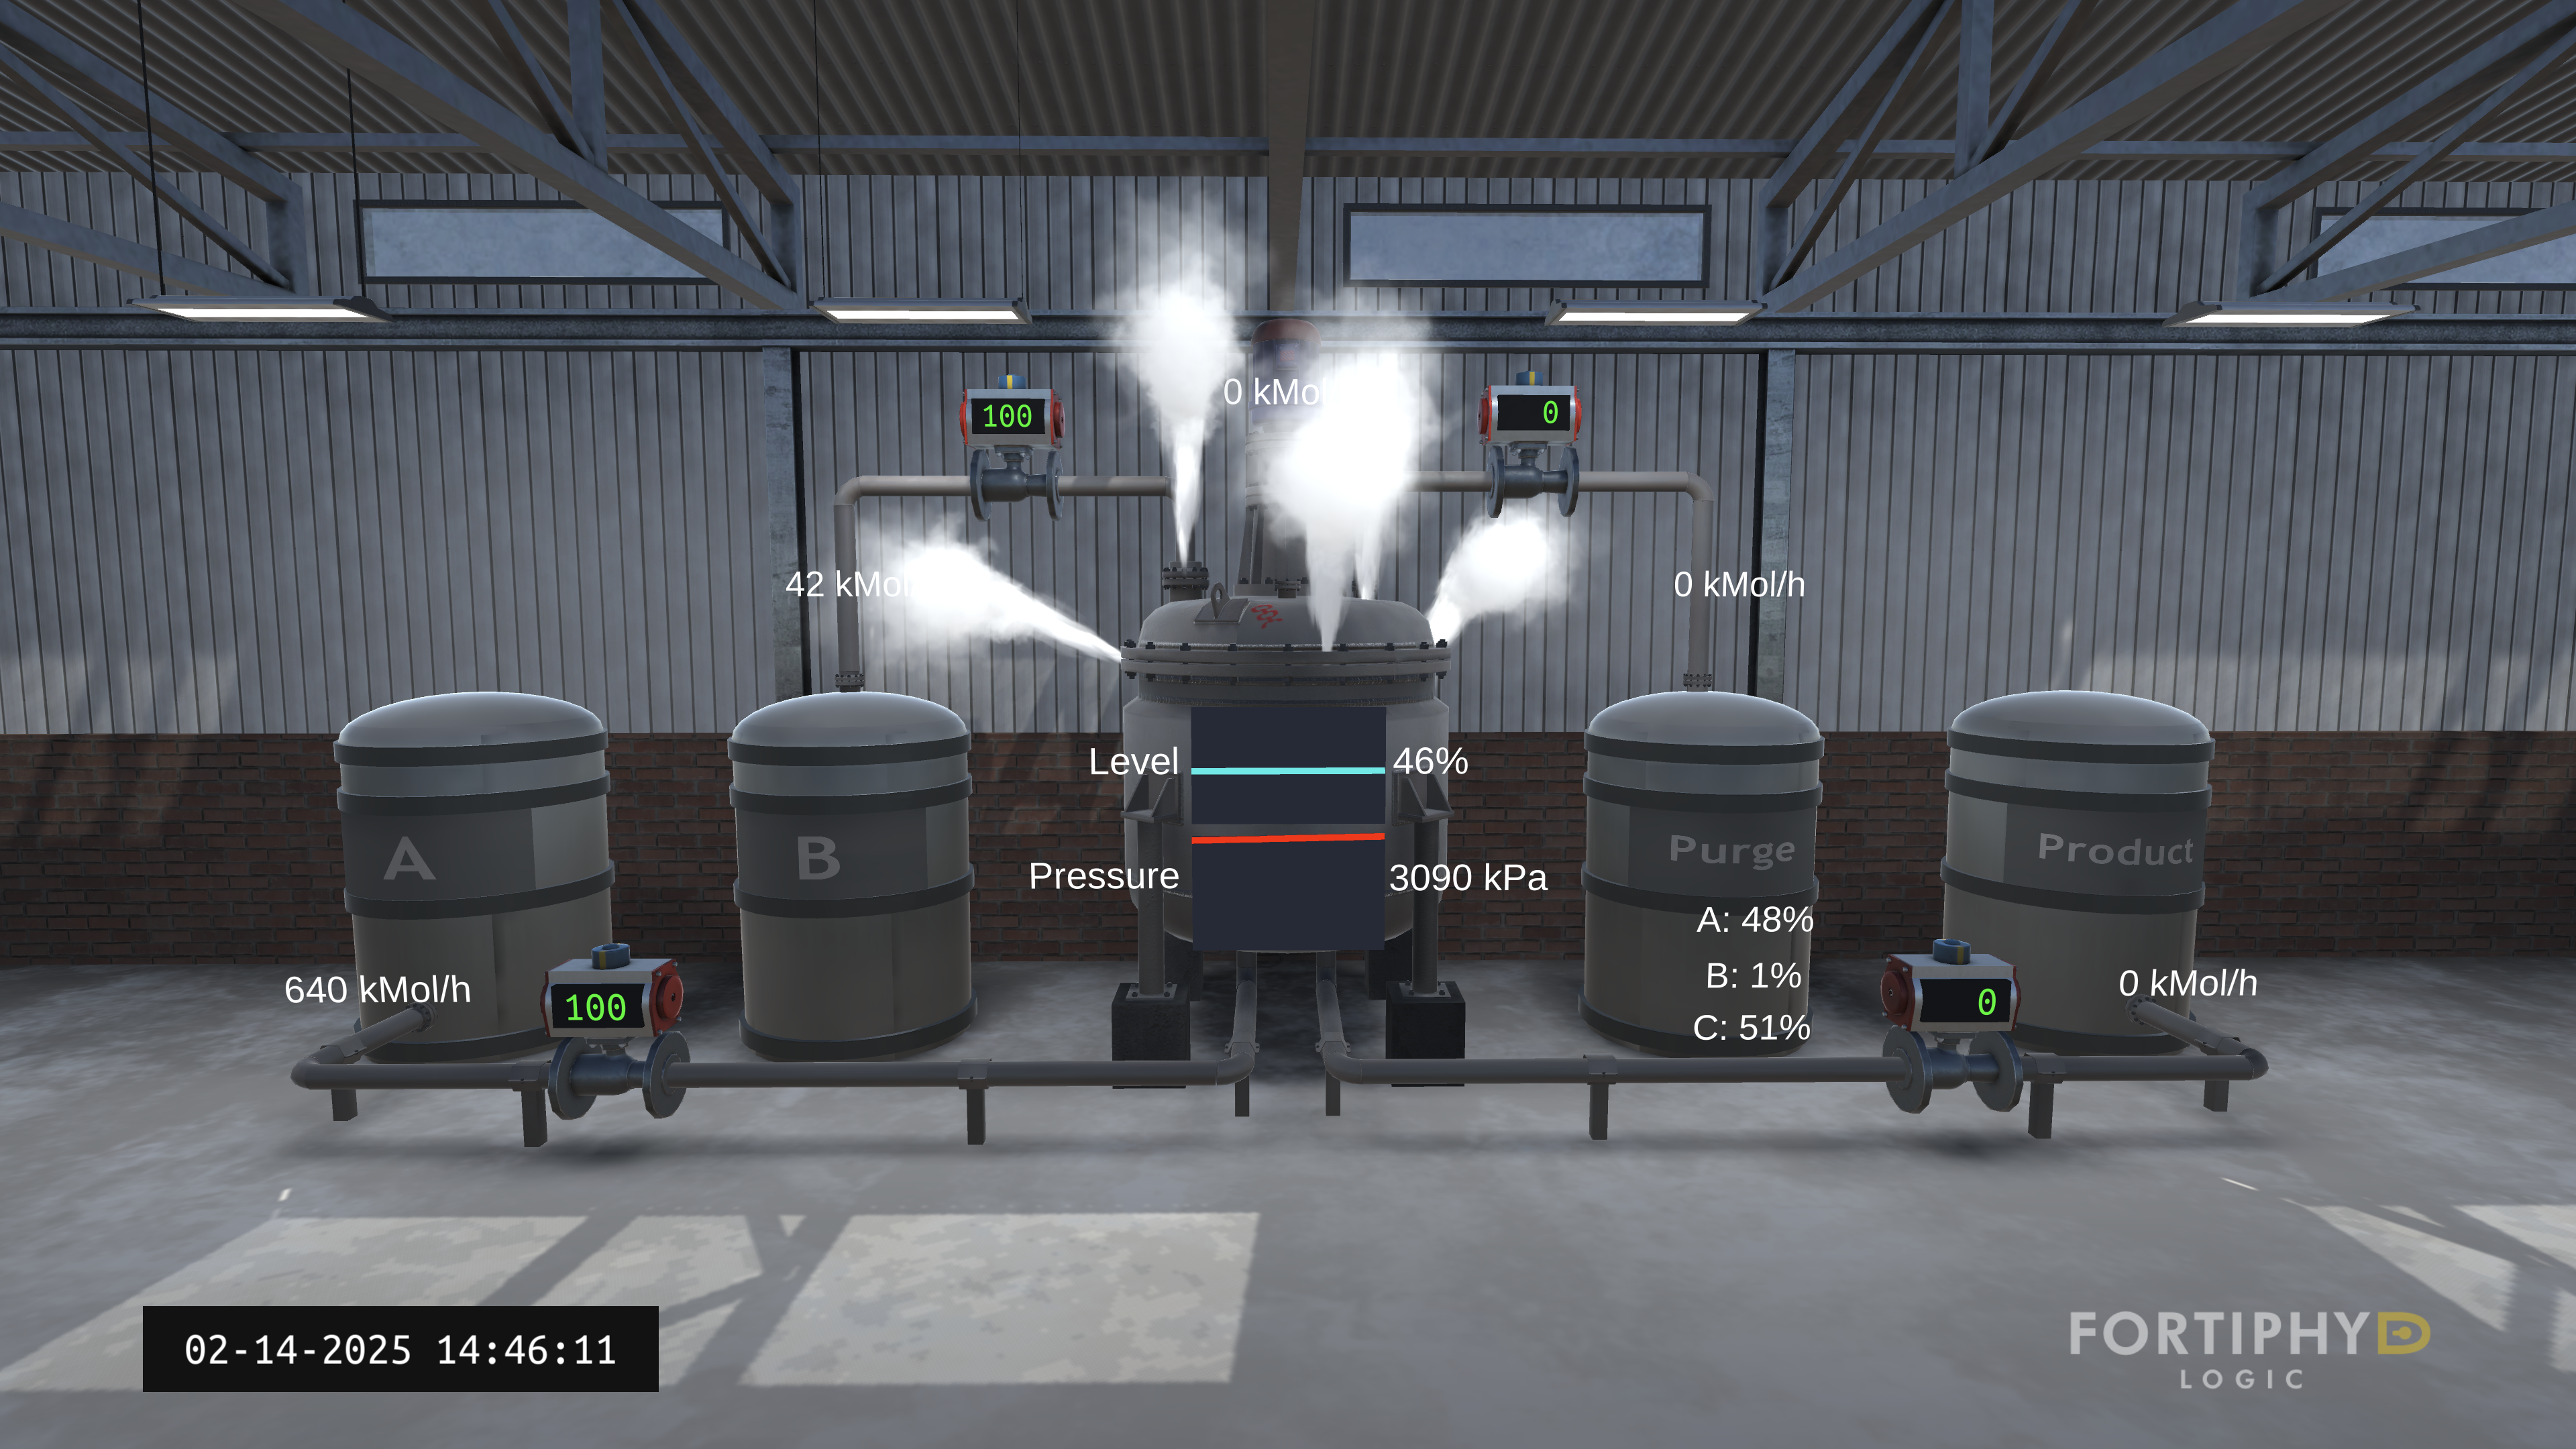
\includegraphics[width=\linewidth,keepaspectratio]{Figures/Stage_3.png}
        % \caption{}
        \label{fig:Stage_3}
    \end{subfigure}
    \hfill % This ensures that there is no additional space between subfigures
    \begin{subfigure}{0.49\linewidth}
\centering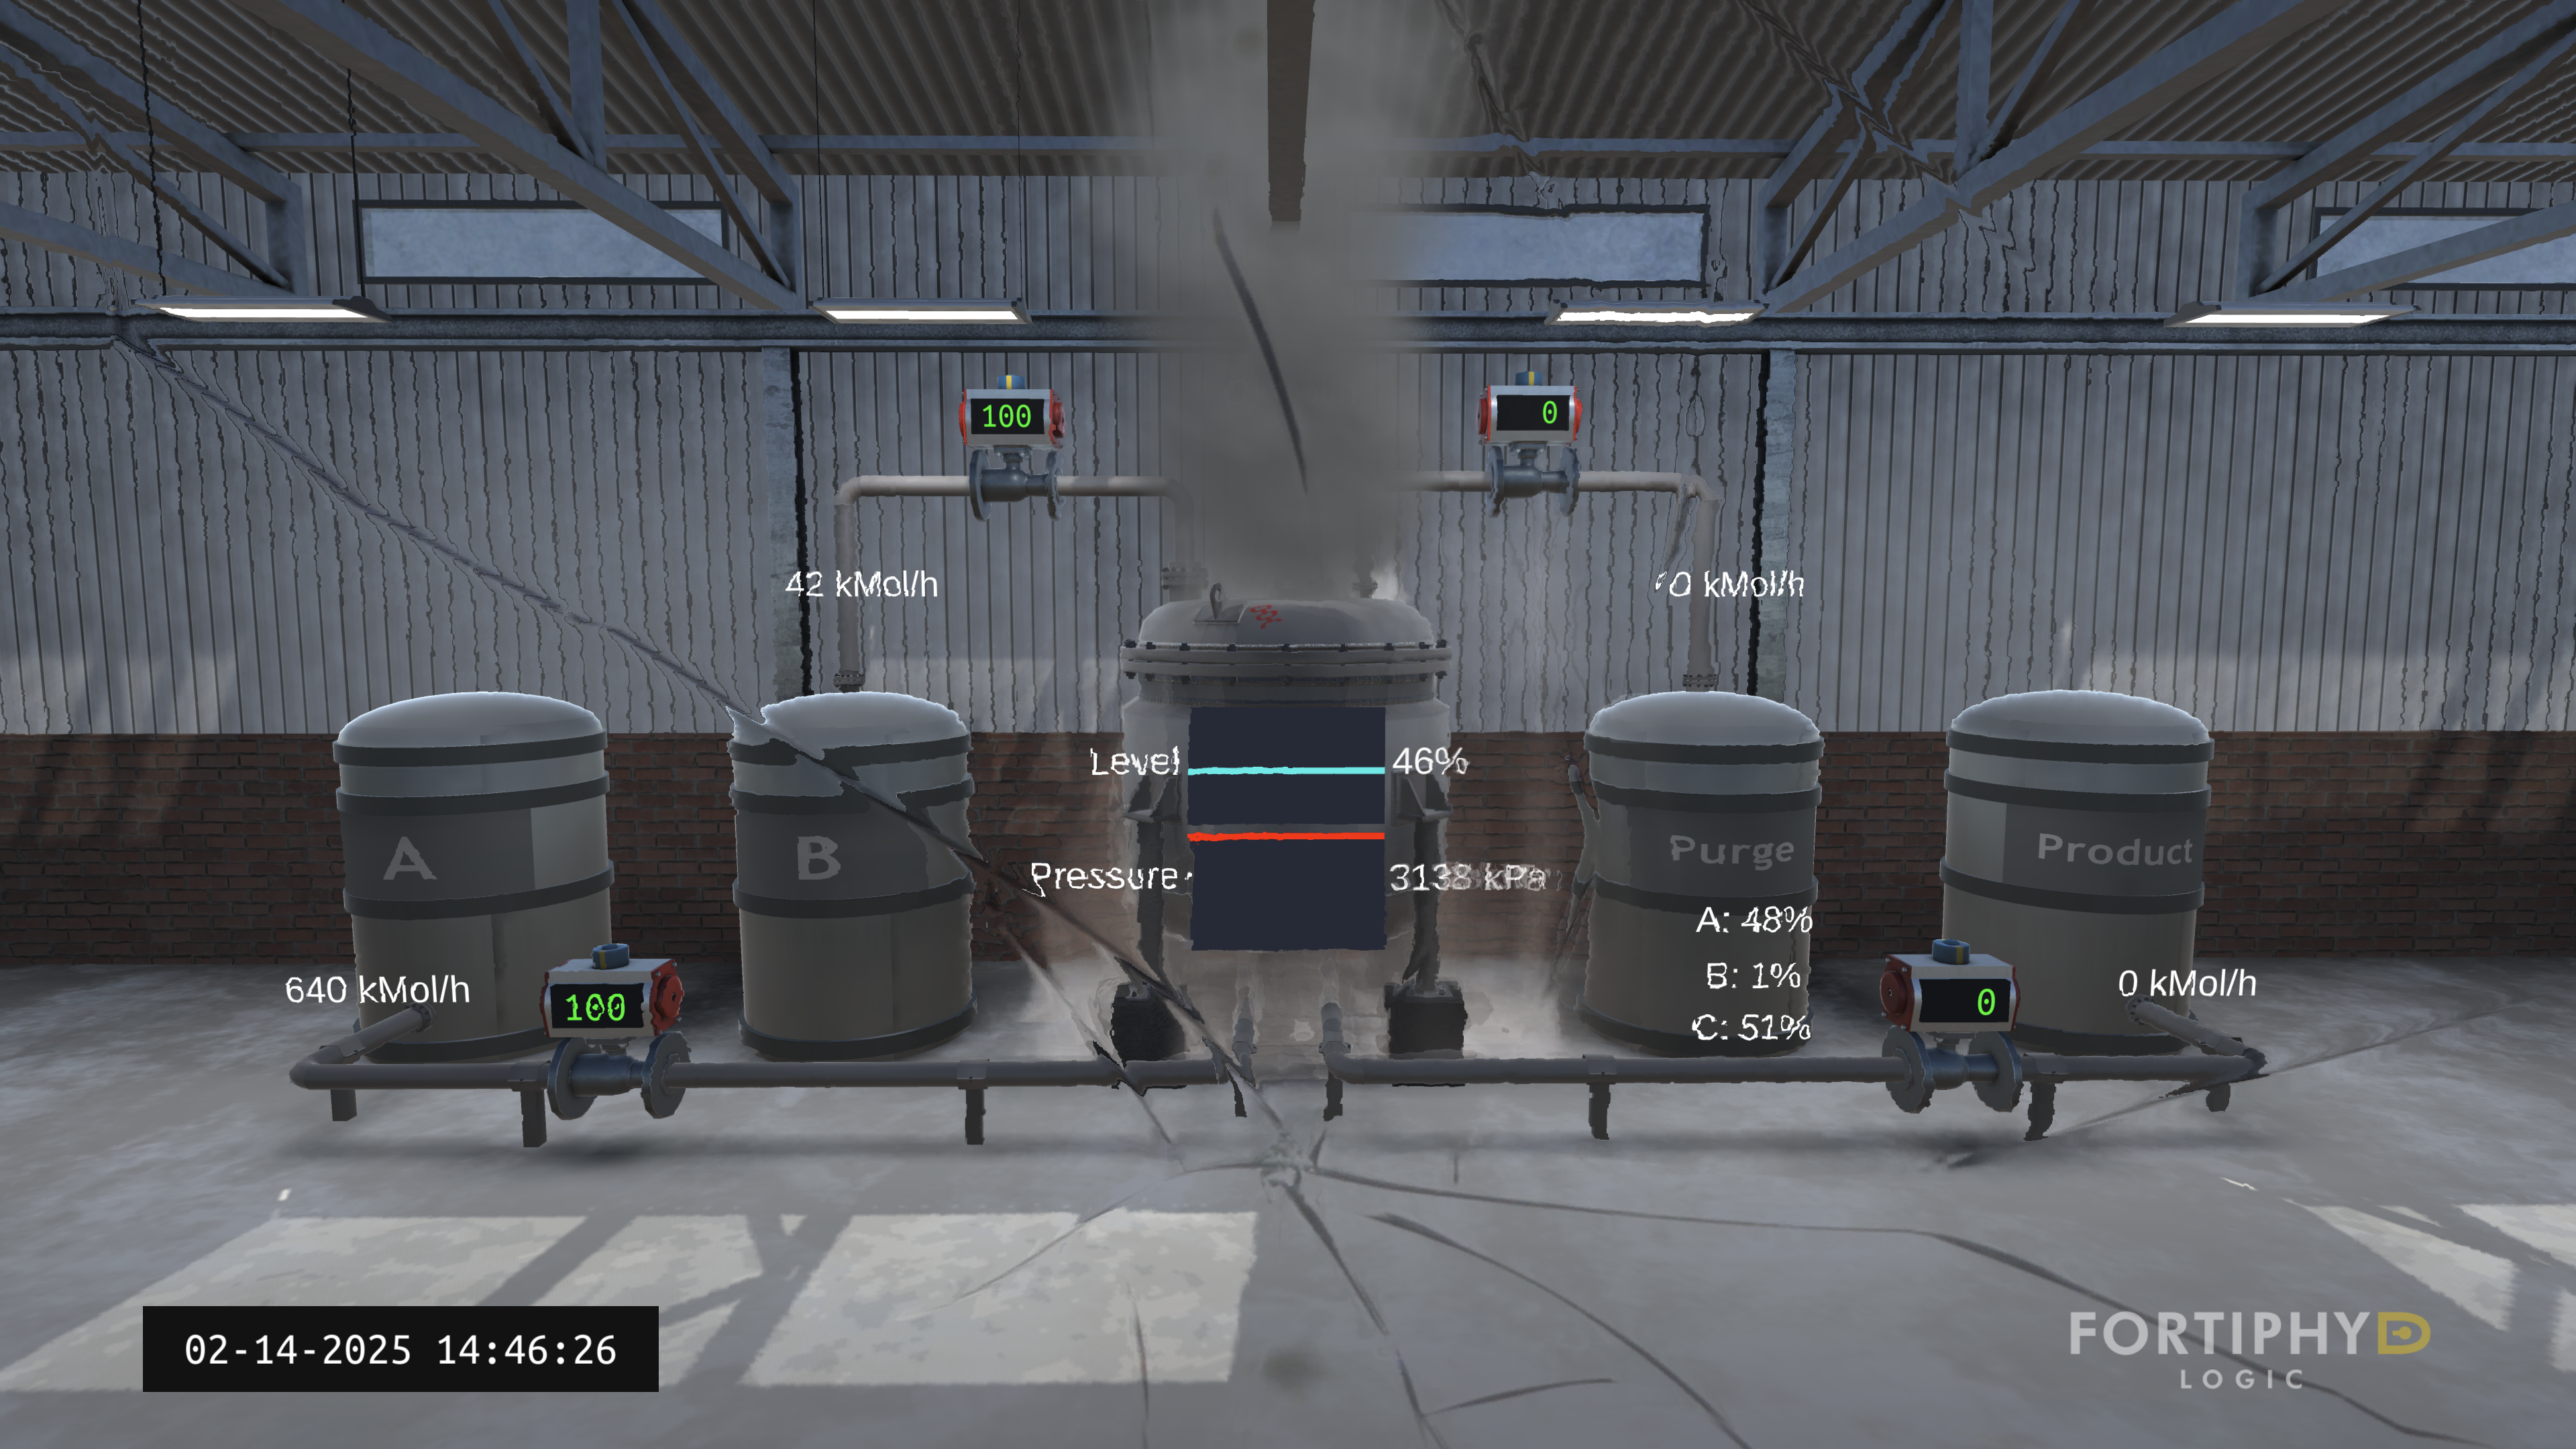
\includegraphics[width=\linewidth,keepaspectratio]{Figures/Stage_5.png}
        % \caption{}
        \label{fig:Stage_5}
    \end{subfigure}
    \begin{subfigure}{\linewidth}
%     \vspace{-0.25cm}
        \centering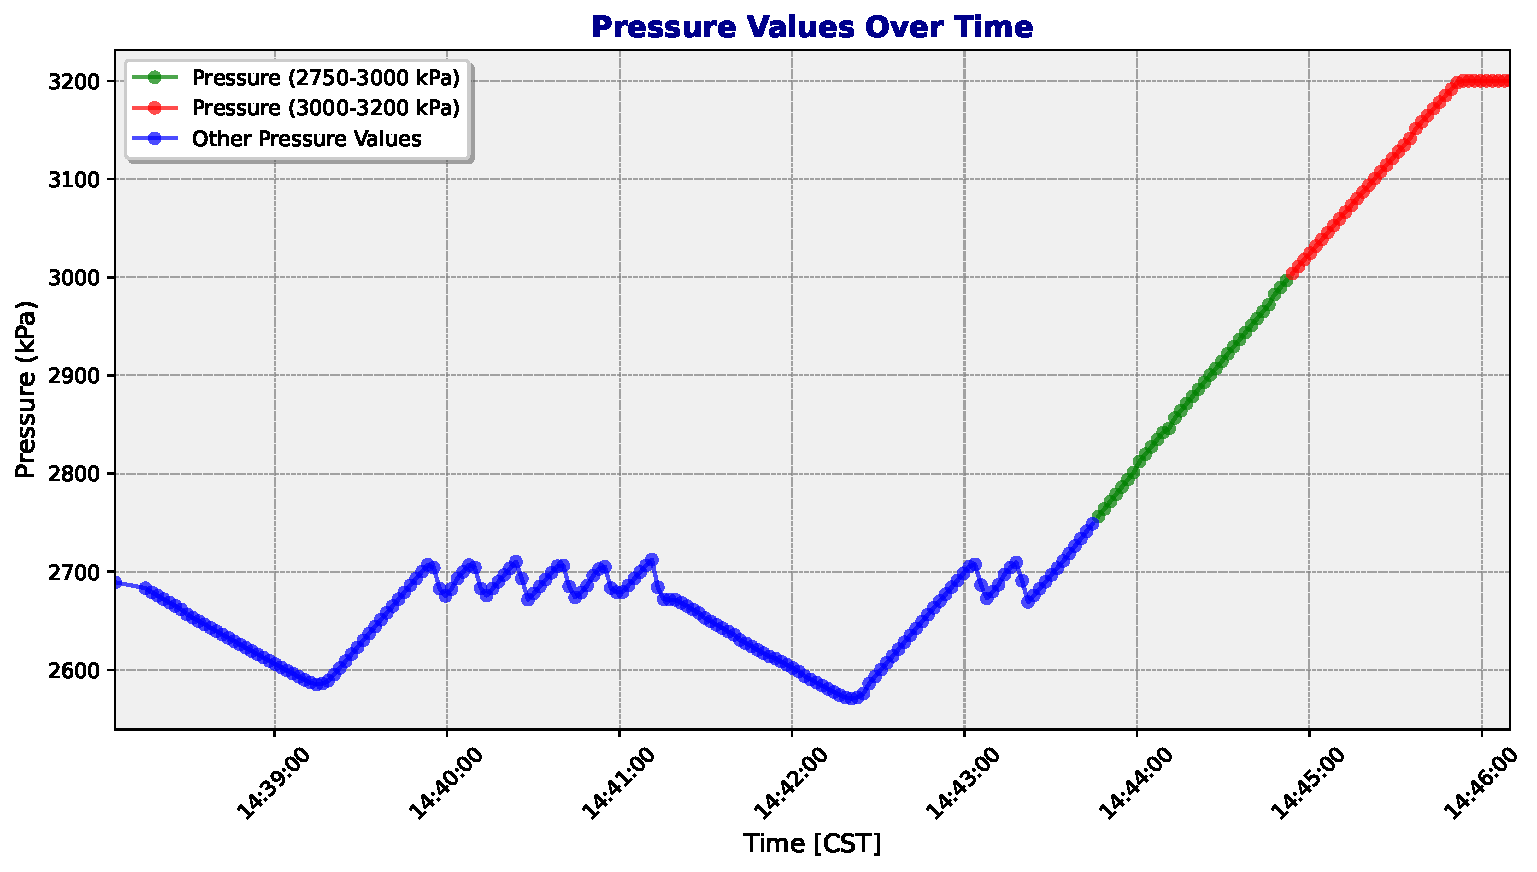
\includegraphics[width=\linewidth,keepaspectratio]{Figures/pressure_plot.pdf}
        % \caption{}
        \label{fig:pressure_plot}
    \end{subfigure}
%     \vspace{-1.25cm}
    \caption{Two different stages in the chemical plant attack emulation showing the instability leading to unavailability of the service. This corresponds to the green and red regions respectively in the pressure plot recorded at the Operator.}
%     \vspace{-0.3cm}
    \label{fig:Chem_figs}
\end{figure}

As described before, the OpenPLC registers hold the values of the setpoint corresponding to different controlled variables of the chemical plant. This control is achieved by regulating the position of the reactants, product, and purge valves based on the user-defined setpoints. The images used in the testbed is set to run the chemical plant at stable values of variables including tank pressure which is set at 2700KPa. There is also a fail-safe value for the pressure beyond which the tank pressure is not allowed to increase which is kept at 2750KPa. These values are written in the registers of the OpenPLC using the SCADA, from where the deployed control algorithm reads and then execute the corresponding control action. We manipulate these setpoints, including the tank pressure, to values higher than the recommended limits. These values are directly written inside the PLC registers, from where the PLC reads it for decision making, thereby taking corrective actions to make the controlled variable reach the desired values. This will cause an increase in pressure and is fatal if left unattended. These changes can be observed from the operator server, where the chemical plant variables are being recorded including the tank pressure. Figure \ref{fig:Chem_figs} shows various stages of the plant before the service unavailability happens.

To understand the effects of DoS attack, we forcefully stop some of the services inside the chemical plant that reports important plant information to the master PLC. We interrupt specifically the Modbus services reporting the measurements of pressure and feed flow (which is a necessary feedback), upon which the controller continues executing the last control action till the desired value is reached. This situation leads to instability due to  the absence of critical feedback, which increases the reaction inside the tank and pushes the pressure beyond safe values. 
% This can be fatal, if the last control action aimed at opening of the feed valves to increase the reaction. 
% In that case, the reaction  will increase inside the tank, making the pressure values go up and thereby pushing the chemical plant to instability. 
The data collected, as shown in the Figure \ref{fig:Chem_figs}, at the Operator server, can help understand the effect of this attack on the Chemical Plant.








